Una schematizzazione dell'apparato usato da Foucault è rappresentato nell'immagine (\ref{App}):\\

\noindent\begin{minipage}{0.5\textwidth}% adapt widths of minipages to your needs
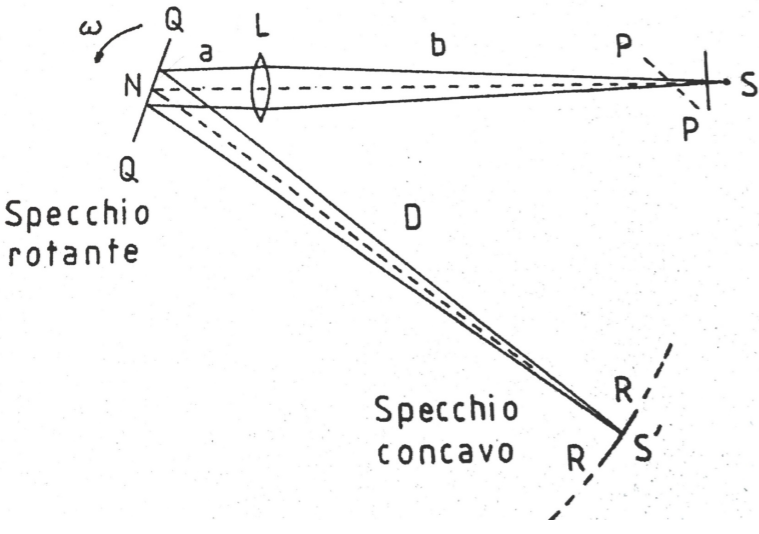
\includegraphics[width=\linewidth]{foucault2.png}
\end{minipage}%
\hfill%
\begin{minipage}{0.5\textwidth}\raggedleft
\begin{itemize}
    \item S è la sorgente luminosa, approssimata puntiforme, da cui parte il fascio luminoso;
    \item Q è uno specchio piano rotante;
    \item R è uno specchio sferico fisso;
    \item L è una lente convergente, tale da convergere il fascio luminoso proveniente da S sul centro dello specchio R;
    \item P è una lastra semitrasparente, necessaria per l'osservazione dei fenomeni
    \item b rappresenta la distanza tra P e L
    \item a rappresenta la distanza tra L e Q
    \item D rappresenta la distanza tra Q ed R
\end{itemize}
\end{minipage}\\



La sorgente luminosa S emette un fascio di luce che, dopo essere stato diaframmato, attraversa una superficie semitrasparente P inclinata di 45° rispetto alla direzione del fascio. Quest'ultimo successivamente attraversa una lente, che porta i raggi luminosi prima a riflettersi nello specchio rotante Q, poi a focalizzarsi sullo specchio concavo R nel punto S', ed infine tornare indietro.
Quando però lo specchio rotante Q viene messo in rotazione a velocità angolare $\omega$, si ha che l'immagine prodotta dalla sorgente S' non coincide più con il raggio di andata: nel tempo necessario affinché la luce compia la distanza D, lo specchio rotante avrà compiuto una rotazione di un angolo $\alpha$ dato da 
\begin{equation}
    \alpha=2(D/c)\omega,
\end{equation}
dove $c$ rappresenta appunto la velocità della luce nell'aria. Il fascio luminoso proveniente da S' viene focalizzato dalla lente L come se provenisse da una sorgente S'', spostata dal S' di una quantità che viene approssimata a 
\begin{equation}
    \Delta=2\alpha D
\end{equation}
essendo l'angolo $\alpha$ sufficientemente piccolo da permettere approssimazioni algebriche senza perdita di significatività.
Una volta attraversata la lente, il fascio luminoso subisce un ingrandimento di modulo pari a 
\begin{equation}
    G=b/(D+a),
\end{equation}
dove $b$ rappresenta la distanza tra la sorgente S e la lente e $a$ indica la distanza tra la lente L e il punto fisso N dello specchio rotante Q.
Sulla lastra semitrasparente P viene dunque uno spostamento $\delta$ pari a 
\begin{equation}
    \delta=G\Delta=\frac{4D^2b\omega}{c(D+a)}
    \label{delta}
\end{equation}

Un problema legato a questa esperienza è quello della luminosità dell'immagine prodotta: l'apparato produce un punto luminoso fintanto che il fascio riflesso dallo specchio rotante colpisce lo specchio concavo. Il rapporto tra la luminosità dell'immagine emessa dalla sorgente S e quella che ritorna sulla lastra semitrasparente P dipende fortemente dalle dimensioni dello specchio concavo e dalla sua apertura. Se la luminosità dell'immagine su P fosse troppo ridotta, non si potrebbe misurare la distanza $\Delta \delta$ e fallirebbe l'esperimento: per ovviare a questo problema, si può scegliere di utilizzare un produttore di raggi laser come sorgente S: l'altissima luminosità di tale raggio garantisce una discreta visibilità del fascio di ritorno. 